


\section{Soundness of our proof system}

\begin{axiom}
We assume a judgment of the form $M \vdash A$, which had the property that\\
\strut \hspace{5cm} $M \vdash A $ \ \ \ \ implies \ \ \ \ $M \vDash A$
\end{axiom}

\subsection{Definitions}

We  define the {\emph {meaning}} of  our Hoare triples, $M\ \vdash\  \{\, A \,  \}\ stmt\  \{\, A' \, \}$,  in the usual way, \ie that execution of $stmt$ in a state that satisfies $A$ leads to a state which satisfies $A'$. 

 
\begin{definition}[Semantics of Hoare triples]

 
For modules $M$, and assertions $A$, $A'$   we define:
%  the semantics of Hoare-triples,   $M\ \models\  \{\, A \,  \}\ stmt\  \{\, A' \, \}$ as follows:
\begin{itemize}
\item
$M\ \models\  \{\, A \,  \}\ stmt\  \{\, A' \, \}$ \\
iff\\
 for   all $\Mtwo$, for all $\sigma$, $\sigma'$ such that {$\arising \sigma {\Mtwo\cdot M}$}\\
$\strut ~ ~ ~ ~ [ \ \ M,\sigma \ \models \ A \ \wedge\  
 \sigma.cont = stmt  \ \wedge\     \leadstoBoundedStarFin {\Mtwo\cdot M}  {\sigma}  {\sigma'}    \ \ \Longrightarrow\ \ M,\sigma' \ \models \ A'\ \ ]$
\end{itemize}
\end{definition}
 

  
 
\subsection{Auxilairy properties of terminating execution} 
 In order to prove the soundness of our proof rules (\ie that $M \models  \{\, A \,  \}\ stmt\  \{\, A' \, \}$ implies that $M \vdash  \{\, A \,  \}\ stmt\  \{\, A' \, \}$, we will need some auxiliary properties of the operational semantics.
 
 The following lemma guarantees that any state reachable from a state with a terminating execution has itself a terminating execution, and that this execution is enclosed in the original one:
 
 \begin{auxLemma}[Enclosed Terminating Executions]\footnote{TODO find better name for the aux lemma}
 For any modules $\Mtwo$,   and states $\sigma$, $\sigma'$, $\sigma_1$:
\begin{itemize}
\item
$  \leadstoBoundedStarFin {\Mtwo}  {\sigma}  {\sigma'} \  \wedge \  \leadstoBoundedStar  {\Mtwo}  {\sigma}  {\sigma_1} 
% $\\ $
\ \ \  \Longrightarrow\ \ \  % $\\ $  
 \exists \sigma_2.[\ \ \leadstoBoundedStarFin {\Mtwo} {\sigma_1}  {\sigma_2}  
\ \wedge\ 
\leadstoBoundedStarThree  {\Mtwo}  {\sigma_2}  {\sigma}   {\sigma'} \ \ ]$
\end{itemize}

\end{auxLemma} 
 
 The following lemma makes the usual guarantee about terminating execution of statement sequences.
  
\begin{auxLemma}[Execution of sequences]
\label{lemma:subexp}
For any modules $\Mtwo$, statements $s_1$, $s_2$, and states $\sigma$, $\sigma'$:
\begin{itemize}
\item
$  \leadstoBoundedStarFin {\Mtwo}  {\sigma}  {\sigma'} \   \wedge\  \sigma.\texttt{cont} = s_1; s_2$\\
$  \Longrightarrow$\\
$   \exists \sigma''.[\ \ \leadstoBoundedStarFin {\Mtwo} {\sigma[\texttt{cont}\mapsto s_1]}  {\sigma''}  
\ \wedge\ 
\leadstoBoundedStarFin {\Mtwo} {\sigma''[\texttt{cont}\mapsto s_2]}   {\sigma'} \ \ ]$
\end{itemize}
\end{auxLemma}
 

 The following lemma says that a terminating execution,  $ \leadstoBoundedStarFin {\Mtwo}  {\sigma}  {\sigma'}$ of an external call   consists of a sequence of  external states interleaved with terminating executions in internal states:
 
\begin{auxLemma}
\label{lemma:external_breakdown}[Summarised External Terminating Execution]
For any module $M$, modules $\Mtwo$, states $\sigma$ and $\sigma'$:
\\
If \\
$\strut \ \ \ \ \ \leadstoBoundedStarFin {M\cdot \Mtwo}  {\sigma}  {\sigma'} \ \ \wedge  \ \ M,\sigma \models \external {\texttt{this}}$
\\
then
\\
$\strut \ \ \ \ \ \exists p,q\in \mathbb{N},  \sigma_1, ... \sigma_q \in States, m_1,...m_p, n_1, ... n_p \in \mathbb{N}.$\\  
$\strut \ \ \ \ \ \ \ \ \ \ [  $ \\
$\strut \ \ \ \ \ \ \ \ \ \  \ \ \ \ \ \ \ \ \sigma_1=\sigma \ \ \wedge\ \  \sigma_p=\sigma'\ \  \wedge\ \ \forall i\in [1..q).[\   \leadstoOrig {M\cdot \Mtwo}  {\sigma_i}  {\sigma_{i+1}}\  ] \  \ \ \wedge$\\
$\strut \ \ \ \ \ \ \ \ \ \  \ \ \ \ \ \ \ \ m_1=1 \ \wedge\ n_p=q+1 \  \wedge\ \forall i\in[1..p).[  \  m_i < n_i < m_{i+1}  ] \ \wedge \ m_p<n_p\ \ \wedge  $\\
$\strut \ \ \ \ \ \ \ \ \ \  \ \ \ \ \ \ \ \ \forall i\in[1..p].\forall j\in [m_i..n_i)[\   M,\sigma_j \models \external {\texttt{this}} \ ] \  \ \ \wedge$\\
$\strut \ \ \ \ \ \ \ \ \ \  \ \ \ \ \ \ \ \ \forall i\in[1..p). [ \ M,\sigma_{n_i} \models \internal {\texttt{this}}   \ \wedge \ \ 
 \leadstoBoundedStarFin {M\cdot \Mtwo}  {\sigma_{n_{i}}}  {\sigma_{m_{i+1}-1}} \ ] $ \\
$\strut \ \ \ \ \ \ \ \ \ \ ]$
\end{auxLemma}

The meaning of Auxialiry lemma \ref{lemma:external_breakdown} is illustrated through an example in Fig. \ref{fig:summaries}.

The following auxiliary lemma describes how an encapsulated assertion $A$ is preserved during an execution, provided that all finalizing internal executions preserved it. 
It will be used in the proof of soundness of the rule {\sc{ExtCall\_WithSpec\_Weak}}\footnoteSD{perhaps also {\sc{ExtCall\_WithSpec\_Strong}}}

\begin{auxLemma}
\label{lemma:external_exec_preserves}[Preservation of Encapsulated Assertions]
For any module $M$, modules $\Mtwo$, numbers $p$ and $q$, states$\sigma_1$, .... $\sigma_p$,  numbers $m_1,...m_p, n_1, ... n_p \in \mathbb{N}$, and assertions $A$:
\\
If \\
$\strut \ \ \ \  M, \sigma_1 \models  A   \  \ \wedge \ \ M \models \encaps A \ \ \ \  \ \ \wedge$\\
$\strut \ \ \ \  \forall i\in [1..q).[\   \leadstoOrig {M\cdot \Mtwo}  {\sigma_i}  {\sigma_{i+1}}\  ] \  \ \ \wedge$\\
$\strut \ \ \ \  m_1=1 \ \wedge\ n_p=q+1 \  \wedge\ \forall i\in[1..p).[  \  m_i < n_i < m_{i+1}  ] \ \wedge \ m_p<n_p\ \ \wedge  $\\
$\strut \ \ \ \  \forall i\in[1..p].\forall j\in [m_i..n_i)[\   M,\sigma_j \models \external {\texttt{this}} \ ] \  \ \ \wedge$\\
$\strut \ \ \ \ \forall i\in[1..p). [ \ M,\sigma_{n_i} \models A   \ \Rightarrow \ \ 
M, {\sigma_{m_{i+1}-1}} \models A  \ ] $ \\
then\\
$\strut \ \ \ \  \ M, \sigma_q \models  A$
\end{auxLemma}



\begin{figure}[htb]
\begin{tabular}{c}
\hline \\
the original execution:
\\
~ \\
\resizebox{9cm}{!}
{
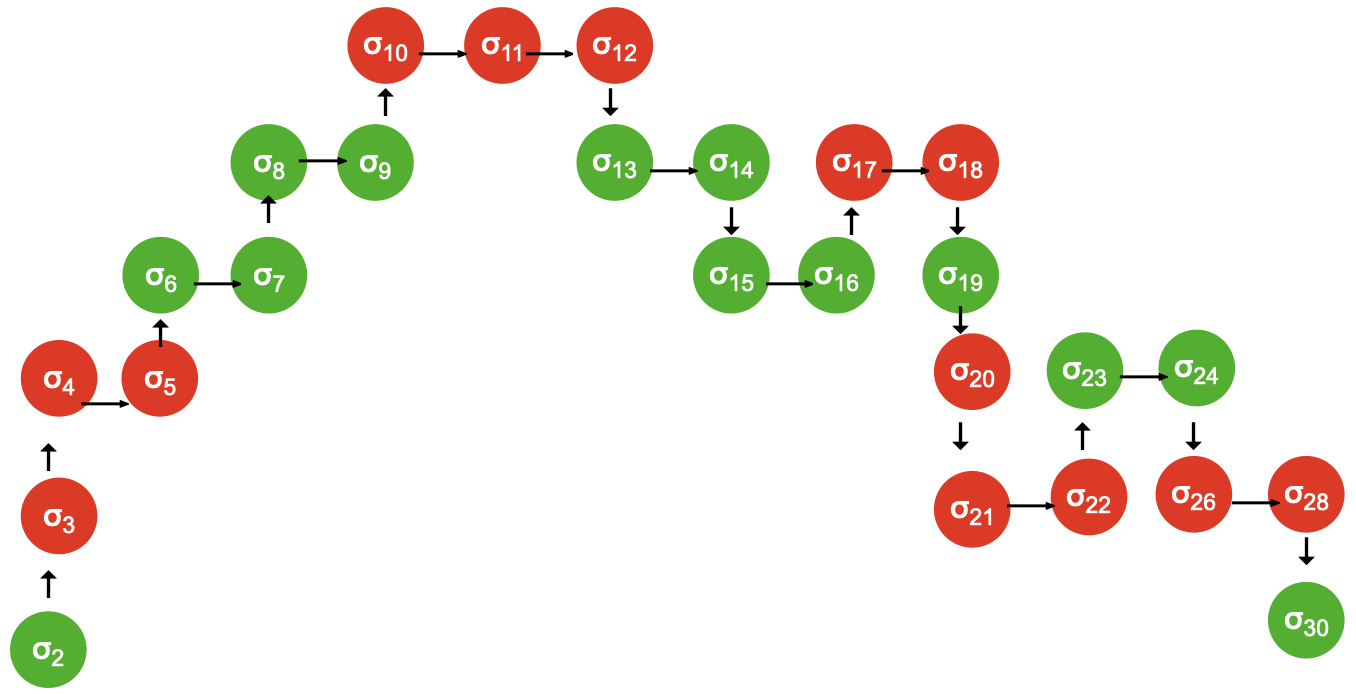
\includegraphics[width=\linewidth]{diagrams/summaryA.png}
} 
\\
\hline \\
the summarised execution:
\\
~ \\
\resizebox{9cm}{!}
{
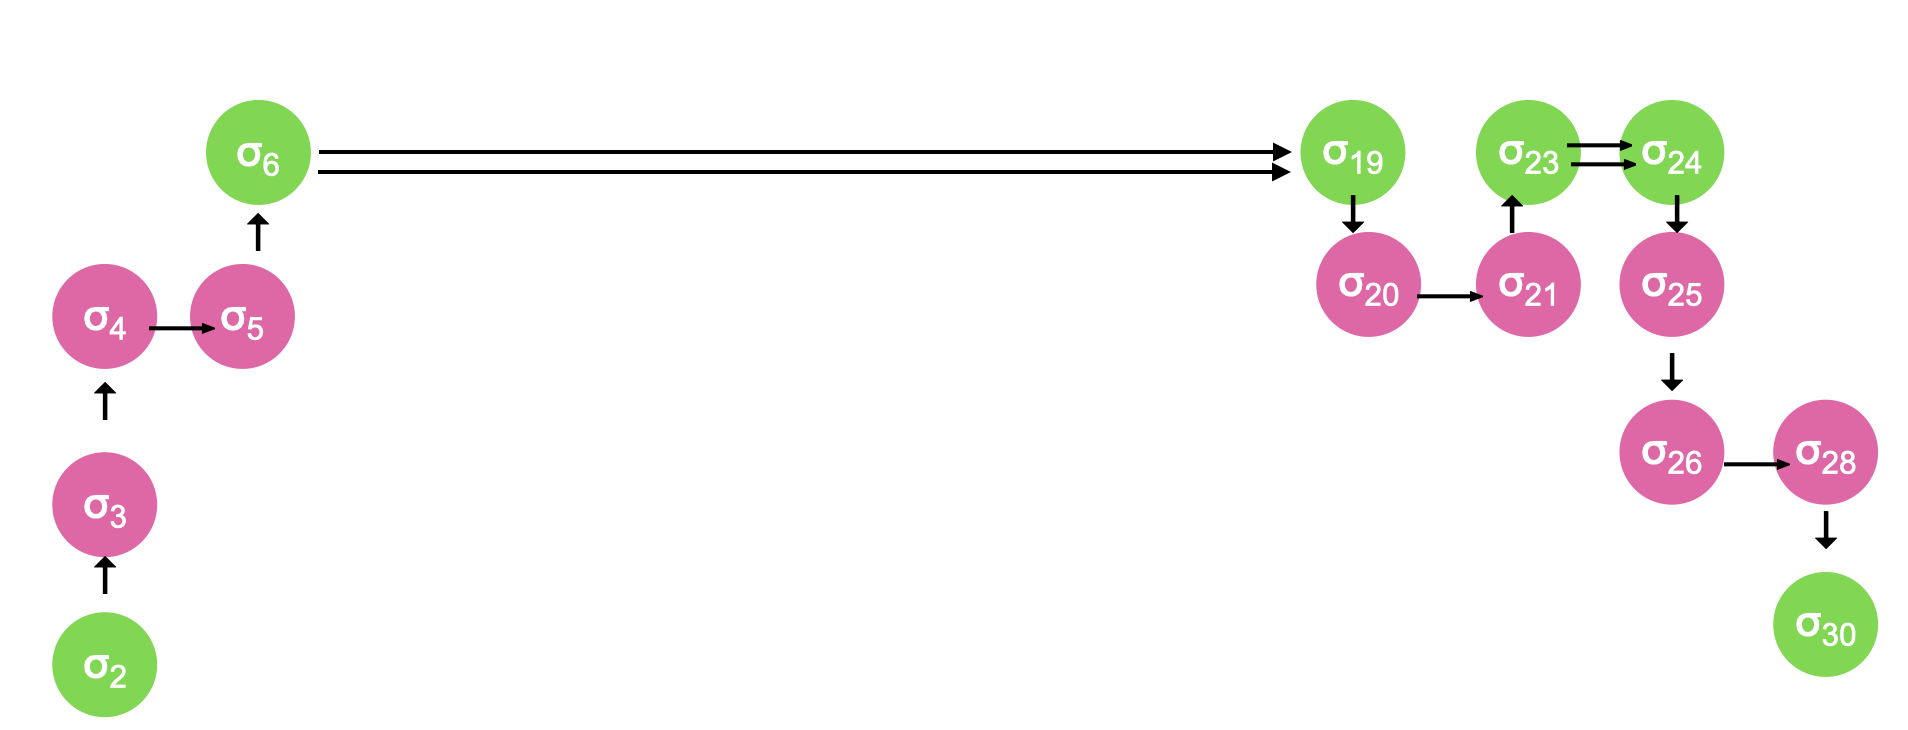
\includegraphics[width=\linewidth]{diagrams/summaryB.png}
} 
\\
\hline \hline
\end{tabular}
   \caption{Summaries. 
   }
   \label{fig:summaries}
 \end{figure}

We now define a well-founded ordering on states, which we will use in the proof of soundness of our Hoare logic. 

\begin{definition}
For module $M$ and states $\sigma$, $\sigma'$, we define
\begin{itemize}
\item $\sigma' \ll_M  \sigma$ \ \ \ iff \ \ \ $\leadstoBoundedStar {M} {\sigma} {\sigma} {\sigma'}$ and $\sigma\neq \sigma'$\\
$\strut \hspace{2cm} \ \ $ or $\\
$\strut \hspace{2cm} \ \ $\sigma.\texttt{cont}=e_1; e_2 \ \ \ \wedge \ \ \ \ \sigma'=\sigma.[\texttt{cont}\mapsto e_1]$
\end{itemize}
\end{definition}

\begin{lemma}
If our language has the acyclic property, then $\ll_M$ is a well-founded ordering.
\end{lemma}

TODO: revisit the lemma above. Need to show that there are no infinite descending chains.

\subsection{Proving Soundness of the Hoare Logic}

We take two modules $M$ and $M'$ arbitrary. We define the following property of states:

$Q(\sigma)\ \ \ \triangleq\  \ \ \forall A, A'. $\\
$\strut \hspace{2cm} [ \  \ Arising(\sigma,M*M') \ \  \wedge\ \ 
% $\\$\strut \hspace{2cm}  \ \ \  \ 
M \vdash \{A \} \sigma.\texttt{cont} \{A' \} \ \ \wedge\ \  M, \sigma \models  A \ \ 
\wedge\ \  \leadstoFin  {M*M'}{\sigma}  {\sigma'}$\\
$\strut \hspace{2cm}   \ \  \Longrightarrow$\\
$\strut \hspace{2cm} \ \   \ \ M, \sigma' \models  A'  \  \ ]$

\noindent
We assume that: \\
$\strut \ \ \ (*) \ \ M \models HS(M)$
where $HS$ also includes Hoare triples for methods.\\
We will prove that \\
$\strut \ \ \ (**) \ \ \forall \sigma.[  \ \ Q(\sigma)\ \ ]$
\\
The proof is by induction on $\sigma$ using the ordering $\ll_{M*M'}$. 

\noindent
\vspace{.2cm}
  {\textbf{Proof Sketch}} 
We start by case analysis on $\sigma.\texttt{cont}$ 

\begin{description} 
\item[$e\ \equiv\ x=y $] 

By standard Hoare logic arguments (or even parametric) ...
\item[$e\ \equiv\ x=y.f $] 

By standard Hoare logic arguments (or even parametric) ...

 \item[$e\ \equiv\ y.m(\overline y)$]  
and $y$ is internal. 

We construct the new frame for the call, $\sigma''$. We obtain that $\sigma'' \ll_{M*M'} \sigma$. We also have that  $ \leadstoFin  {M*M'}{\sigma''}  {\sigma'}$, and $\sigma''$ "returns to $\sigma'$.
We apply the IH to $\sigma''$ and knowledge from Hoare loci rules, and are done.  

\item[$e\ \equiv\ y.m(\overline y)$]  and $y$ is external. 
\\
We apply the rule for external calls, and obtain that the argument hinges on a requirement that there is an invariant property $A''$, which is lifted to the first external call, and will we need to demonstrate is preserved by al enclosed call internal or external, and this $A''$ must be valid at the last external frame, and is then lowered to the current frame.
\\
We apply lemma \ref{lemma:external_breakdown}. In terms of the example in Fig. \ref{fig:summaries} we are now working with the summarised execution, \ie the execution of the methods in $\sigma_8$ and 
$\sigma_{22}$ is summarised into one large step.
Regardless of example, obtain that the first external calls ($\sigma_2$, ... $\sigma_{j_2}$) all preserve $A''$ because it is encapsulated. 
Therefore $A''$ also holds at $\sigma_{j_2}+1$. 
Since we have (*), we know that $A''$ has been proven as an invariant of all external methods, and therefore, by applying the (H), we obtain that $A''$ holds at $\sigma_{j_2} + 3$  (In terms of our example in Fig. \ref{fig:summaries}  $A''$ would hold in $\sigma_{24}).$ 
We continue in the same vain, until we reach $\sigma_{n-1}$ (that is $\sigma_{28}$ in our example), and then we apply the Hoare rule and what we know about lowering.
 \item[$e\ \equiv e_1; e_2$ ]
 By lemma \ref{lemma:subexp} we can break execution to two parts. For the second part we can apply the IH. But for the first part is looks as if we are repeating the work from earlier cases. OR... should we extend the def of $\\ll_M$ so that $\sigma[\texttt{cont}\mapsto e_1] \ll_M \sigma$.
\end{description}


\vspace{1cm}

Finally, we can now prove soundness of the overall system

\begin{theorem}[Soundness]
\label{thm:soundness}
Assume a a sound \SpecO proof system, $\proves{M}{A}$, 
a sound encapsulation inference system, $\proves{M}{\encaps{A}}$,
 and  that on top of these systems we built
 the \SpecLang logic according to the rules in Figures \ref{f:classical->singlestep},  \ref{f:only-if-single}, 
 \ref{f:only-through},  and \ref{f:only-if},   then, for    all modules $M$, and all \SpecLang specifications  $S$:
 
 $$\proves{M}{S}\ \ \ \ \ \ \ \mbox{implies}\ \ \ \ \ \  \ \ \ \satisfies{M}{S}$$
\end{theorem}

\begin{proof}
follows from earlier theorem
% by induction on the derivation of $\proves{M}{S}$.
\end{proof}
 


Theorem. \ref{thm:soundness} demonstrates 
 that the   \SpecLang logic is sound with respect to the semantics of \SpecLang specifications.
 The \SpecLang logic parametric wrt to the algorithms for proving validity of assertions
 $\proves{M}{A}$, and 
 assertion encapsulation ($\proves{M}{\encaps{A}}$), and is sound
 provided that these two proof systems are sound.

